\documentclass[conference]{IEEEtran}
\IEEEoverridecommandlockouts
\usepackage[T1]{fontenc}
\usepackage{amsmath,amsthm}
\usepackage{newtxtext,newtxmath}
\usepackage{booktabs}
\usepackage{graphicx}
\usepackage{cite}
\usepackage{url}
\usepackage{xcolor}
\usepackage{algorithm}
\usepackage{algpseudocode}

% Auto-generated by plots/make_paper_assets.py -- do not edit.
\newcommand{\AbsCoeff}{1.54}
\newcommand{\AbsDbKm}{6.68}
\newcommand{\AssocAllOptimalStatus}{yes}
\newcommand{\AssocCertPct}{82.3}
\newcommand{\AssocInstances}{1800}
\newcommand{\AssocLpMaxGap}{3}
\newcommand{\AssocLpSlotMaxGap}{2}
\newcommand{\AssocLpSlotTightPct}{94.8}
\newcommand{\AssocLpTightPct}{35.7}
\newcommand{\AssocMaxGap}{7}
\newcommand{\AssocMaxGapText}{7 users}
\newcommand{\AssocOptimalPct}{84.1}
\newcommand{\AssocPaceMaxGap}{2}
\newcommand{\AssocPaceMaxGapText}{2 users}
\newcommand{\AssocPaceOptimalPct}{99.4}
\newcommand{\AssocPaceWorstRatio}{96.6}
\newcommand{\AssocPerDemand}{360}
\newcommand{\AssocShortGreedy}{483}
\newcommand{\AssocShortPace}{12}
\newcommand{\AssocShortReduction}{97.5}
\newcommand{\AssocTExact}{34.0}
\newcommand{\AssocTExactPnn}{469.8}
\newcommand{\AssocTGreedy}{0.27}
\newcommand{\AssocTGreedyPnn}{0.60}
\newcommand{\AssocTPace}{0.62}
\newcommand{\AssocTPacePnn}{15.81}
\newcommand{\AssocWins}{282}
\newcommand{\AssocWorstRatio}{87.0}
\newcommand{\BudgetUnit}{1600}
\newcommand{\CommissionedCov}{100.0}
\newcommand{\DispReductionVsGa}{18.8}
\newcommand{\EscCertPct}{98.7}
\newcommand{\EscN}{457}
\newcommand{\ExposureHalfMeter}{0.69}
\newcommand{\FlatBudget}{6400}
\newcommand{\FpsoDisp}{22.4}
\newcommand{\FpsoLat}{30.5}
\newcommand{\FpsoMoved}{13.2}
\newcommand{\FpsoPD}{0.36}
\newcommand{\FpsoPS}{$<10^{-4}$}
\newcommand{\FpsoPw}{0.45}
\newcommand{\FpsoRt}{22.9}
\newcommand{\FpsoS}{78.3}
\newcommand{\FpsoSCI}{2.5}
\newcommand{\FpsoSleep}{4.4}
\newcommand{\FpsoThz}{42.5}
\newcommand{\FpsoWifi}{4.0}
\newcommand{\GaDisp}{30.4}
\newcommand{\GaLat}{40.1}
\newcommand{\GaMoved}{12.5}
\newcommand{\GaPD}{0.005}
\newcommand{\GaPS}{0.02}
\newcommand{\GaPw}{0.61}
\newcommand{\GaRt}{25.0}
\newcommand{\GaS}{87.3}
\newcommand{\GaSCI}{2.7}
\newcommand{\GaSleep}{3.9}
\newcommand{\GaThz}{47.8}
\newcommand{\GaWifi}{4.0}
\newcommand{\GainOneTwenty}{7.4}
\newcommand{\GainSixty}{10.4}
\newcommand{\GainThirty}{13.4}
\newcommand{\GainVsStatic}{39.6}
\newcommand{\GainVsThz}{7.2}
\newcommand{\GainVsTm}{33.5}
\newcommand{\GapToGa}{2.9}
\newcommand{\GapVsNaiveA}{1.8}
\newcommand{\GapVsNaiveB}{2.0}
\newcommand{\GapVsNaiveC}{1.5}
\newcommand{\GapVsNaiveD}{0.9}
\newcommand{\GapVsNaiveE}{-0.1}
\newcommand{\GapVsNaivePA}{$<10^{-4}$}
\newcommand{\GapVsNaivePB}{$<10^{-5}$}
\newcommand{\GapVsNaivePC}{$<10^{-3}$}
\newcommand{\GapVsNaivePD}{$<10^{-3}$}
\newcommand{\GapVsNaivePE}{0.64}
\newcommand{\GreedyDisp}{24.6}
\newcommand{\GreedyDispA}{4.5}
\newcommand{\GreedyDispB}{16.1}
\newcommand{\GreedyDispC}{18.7}
\newcommand{\GreedyDispD}{22.4}
\newcommand{\GreedyDispE}{26.1}
\newcommand{\GreedyElecA}{78}
\newcommand{\GreedyElecB}{30}
\newcommand{\GreedyElecC}{19}
\newcommand{\GreedyElecD}{2}
\newcommand{\GreedyElecE}{0}
\newcommand{\GreedyLat}{37.6}
\newcommand{\GreedyMoved}{12.6}
\newcommand{\GreedyPD}{0.18}
\newcommand{\GreedyPS}{0.65}
\newcommand{\GreedyPw}{0.53}
\newcommand{\GreedyRt}{22.6}
\newcommand{\GreedyS}{84.4}
\newcommand{\GreedySCI}{2.6}
\newcommand{\GreedySleep}{4.1}
\newcommand{\GreedyThz}{46.1}
\newcommand{\GreedyWifi}{4.0}
\newcommand{\HpsoDisp}{13.5}
\newcommand{\HpsoLat}{18.8}
\newcommand{\HpsoMoved}{12.2}
\newcommand{\HpsoPD}{$<10^{-7}$}
\newcommand{\HpsoPS}{$<10^{-6}$}
\newcommand{\HpsoPw}{0.43}
\newcommand{\HpsoRt}{22.4}
\newcommand{\HpsoS}{75.0}
\newcommand{\HpsoSCI}{2.5}
\newcommand{\HpsoSleep}{4.5}
\newcommand{\HpsoThz}{40.5}
\newcommand{\HpsoWifi}{4.0}
\newcommand{\LayoutSeedCov}{85.5}
\newcommand{\LegacyCovCompass}{60.8}
\newcommand{\LegacyCovMath}{43.9}
\newcommand{\MainSeeds}{30}
\newcommand{\MainUsers}{59.3}
\newcommand{\MaxEirp}{33.4}
\newcommand{\MilpCovCorrected}{66.2}
\newcommand{\NaiveDisp}{23.3}
\newcommand{\NaiveLat}{34.6}
\newcommand{\NaiveMoved}{12.1}
\newcommand{\NaivePD}{0.09}
\newcommand{\NaivePS}{0.010}
\newcommand{\NaivePw}{0.51}
\newcommand{\NaiveRt}{23.7}
\newcommand{\NaiveS}{83.0}
\newcommand{\NaiveSCI}{2.8}
\newcommand{\NaiveSleep}{4.3}
\newcommand{\NaiveThz}{45.4}
\newcommand{\NaiveWifi}{3.9}
\newcommand{\NoiseThz}{-64.0}
\newcommand{\NomoveDisp}{0.0}
\newcommand{\NomoveLat}{0.0}
\newcommand{\NomoveMoved}{0.0}
\newcommand{\NomovePD}{$<10^{-8}$}
\newcommand{\NomovePS}{$<10^{-8}$}
\newcommand{\NomovePw}{0.36}
\newcommand{\NomoveRt}{5.5}
\newcommand{\NomoveS}{58.9}
\newcommand{\NomoveSCI}{2.6}
\newcommand{\NomoveSleep}{4.9}
\newcommand{\NomoveThz}{30.9}
\newcommand{\NomoveWifi}{4.0}
\newcommand{\NopcDisp}{24.7}
\newcommand{\NopcLat}{37.6}
\newcommand{\NopcMoved}{12.6}
\newcommand{\NopcPD}{1.00}
\newcommand{\NopcPS}{1.00}
\newcommand{\NopcPw}{1.40}
\newcommand{\NopcRt}{24.5}
\newcommand{\NopcS}{84.4}
\newcommand{\NopcSCI}{2.6}
\newcommand{\NopcSleep}{0.0}
\newcommand{\NopcThz}{46.1}
\newcommand{\NopcWifi}{4.0}
\newcommand{\PaceDispA}{3.8}
\newcommand{\PaceDispB}{15.5}
\newcommand{\PaceDispC}{19.1}
\newcommand{\PaceDispD}{22.3}
\newcommand{\PaceDispE}{25.8}
\newcommand{\PaceElecA}{80}
\newcommand{\PaceElecB}{33}
\newcommand{\PaceElecC}{20}
\newcommand{\PaceElecD}{2}
\newcommand{\PaceElecE}{0}
\newcommand{\PaceRtRatioA}{2.5}
\newcommand{\PaceSGainA}{0.3}
\newcommand{\PaceSGainB}{0.1}
\newcommand{\PaceSGainC}{0.2}
\newcommand{\PaceSGainD}{0.1}
\newcommand{\PaceSGainE}{-0.1}
\newcommand{\PaceSPA}{0.01}
\newcommand{\PaceSPB}{0.40}
\newcommand{\PaceSPC}{0.25}
\newcommand{\PaceSPD}{0.09}
\newcommand{\PaceSPE}{0.80}
\newcommand{\PaceSPMinRest}{0.09}
\newcommand{\PaceTzeroGainA}{1.0}
\newcommand{\PaceTzeroGainB}{0.4}
\newcommand{\PaceTzeroGainC}{0.5}
\newcommand{\PaceTzeroGainD}{0.0}
\newcommand{\PaceTzeroGainE}{0.0}
\newcommand{\PowerSaving}{62.1}
\newcommand{\PropDisp}{24.7}
\newcommand{\PropLat}{37.6}
\newcommand{\PropMoved}{12.6}
\newcommand{\PropPw}{0.53}
\newcommand{\PropRt}{24.6}
\newcommand{\PropS}{84.4}
\newcommand{\PropSCI}{2.6}
\newcommand{\PropSleep}{4.0}
\newcommand{\PropThz}{46.1}
\newcommand{\PropTzero}{51.6}
\newcommand{\PropWifi}{4.0}
\newcommand{\RegimeDispRatio}{23.7}
\newcommand{\RegimeElecHighDemand}{0}
\newcommand{\RegimeElecLowDemand}{80}
\newcommand{\RegimeElecMax}{100}
\newcommand{\RegimeSLowDemand}{98.3}
\newcommand{\RegimeSMax}{100.0}
\newcommand{\RegimeSMin}{62.6}
\newcommand{\RegimeTzeroHigh}{41.7}
\newcommand{\RegimeTzeroLow}{94.2}
\newcommand{\SensHalf}{63.6}
\newcommand{\SensOne}{62.8}
\newcommand{\SensQuarter}{68.0}
\newcommand{\SensZero}{84.4}
\newcommand{\StaticDisp}{0.0}
\newcommand{\StaticLat}{0.0}
\newcommand{\StaticMoved}{0.0}
\newcommand{\StaticPD}{$<10^{-8}$}
\newcommand{\StaticPS}{$<10^{-5}$}
\newcommand{\StaticPw}{1.40}
\newcommand{\StaticRt}{0.0}
\newcommand{\StaticS}{44.8}
\newcommand{\StaticSCI}{3.1}
\newcommand{\StaticSleep}{0.0}
\newcommand{\StaticThz}{26.7}
\newcommand{\StaticWifi}{0.0}
\newcommand{\TCumReduction}{20.3}
\newcommand{\TEpochs}{6}
\newcommand{\TGaCum}{97.2}
\newcommand{\TGaHo}{31.8}
\newcommand{\TGaHv}{9.3}
\newcommand{\TGaPw}{0.63}
\newcommand{\TGaS}{90.1}
\newcommand{\TPropCum}{77.5}
\newcommand{\TPropHo}{31.7}
\newcommand{\TPropHv}{9.7}
\newcommand{\TPropPw}{0.58}
\newcommand{\TPropS}{87.9}
\newcommand{\TStaticCum}{0.0}
\newcommand{\TStaticHo}{11.2}
\newcommand{\TStaticHv}{0.0}
\newcommand{\TStaticPw}{1.40}
\newcommand{\TStaticS}{43.0}
\newcommand{\TTmCum}{61.7}
\newcommand{\TTmHo}{18.1}
\newcommand{\TTmHv}{0.0}
\newcommand{\TTmPw}{1.40}
\newcommand{\TTmS}{53.9}
\newcommand{\ThzDisp}{25.8}
\newcommand{\ThzLat}{38.9}
\newcommand{\ThzMoved}{12.5}
\newcommand{\ThzPD}{0.92}
\newcommand{\ThzPS}{$<10^{-5}$}
\newcommand{\ThzPw}{0.55}
\newcommand{\ThzRt}{23.4}
\newcommand{\ThzS}{77.2}
\newcommand{\ThzSCI}{2.5}
\newcommand{\ThzSleep}{4.2}
\newcommand{\ThzThz}{45.9}
\newcommand{\ThzWifi}{0.0}
\newcommand{\TmDisp}{11.8}
\newcommand{\TmLat}{15.6}
\newcommand{\TmMoved}{13.4}
\newcommand{\TmPD}{$<10^{-5}$}
\newcommand{\TmPS}{$<10^{-8}$}
\newcommand{\TmPw}{1.40}
\newcommand{\TmRt}{70.2}
\newcommand{\TmS}{50.9}
\newcommand{\TmSCI}{2.5}
\newcommand{\TmSleep}{0.0}
\newcommand{\TmThz}{30.3}
\newcommand{\TmWifi}{0.0}
\newcommand{\TzeroCertPct}{78.0}
\newcommand{\UePsi}{10.9}
\newcommand{\WifiDisp}{0.0}
\newcommand{\WifiGainHigh}{-0.4}
\newcommand{\WifiGainLow}{22.7}
\newcommand{\WifiLat}{0.0}
\newcommand{\WifiMaxRate}{1.68}
\newcommand{\WifiMoved}{0.0}
\newcommand{\WifiPD}{$<10^{-8}$}
\newcommand{\WifiPS}{$<10^{-5}$}
\newcommand{\WifiPw}{0.00}
\newcommand{\WifiRt}{0.0}
\newcommand{\WifiS}{6.8}
\newcommand{\WifiSCI}{0.2}
\newcommand{\WifiSleep}{14.0}
\newcommand{\WifiThz}{0.0}
\newcommand{\WifiWifi}{4.0}


\newtheorem{proposition}{Proposition}
\newcommand{\Rmin}{R_{\min}}
\newcommand{\Pmax}{P_{\max}}

\begin{document}

\title{TeraMove-H: Crowd-Aware Association, Power Control and Reconfiguration of Movable THz Access Points in Hybrid THz/Wi-Fi Indoor Networks}

\author{\IEEEauthorblockN{Author 1, Author 2, Author 3}
\IEEEauthorblockA{Department of Computer Science and Engineering, Indian Institute of Technology Bhilai, India}}

\maketitle

\begin{abstract}
Indoor terahertz (THz) access points (APs) need line of sight, so the people they serve are also what blocks them.
Earlier work places APs with a mixed-integer program and moves them with a tiered swarm optimizer when crowds degrade coverage.
We extend this line of work to a hybrid network in which fixed Wi-Fi APs coexist with movable THz APs, and we add two electronic control steps that run before any hardware moves.
First, user association is posed as a maximum generalized assignment problem under per-AP airtime budgets.
We solve it with PACE, a Lagrangian airtime-pricing algorithm with ejection chains.
PACE reaches the exact optimum in \AssocPaceOptimalPct\% of \AssocInstances{} test instances, against \AssocOptimalPct\% for a greedy, and certifies optimality in \AssocCertPct\% of them.
Second, a minimum-power control step, based on Yates' standard interference functions, switches idle THz APs off and lowers transmit power without losing any served user.
Only when these steps fail does the network re-steer beams and, finally, move APs along per-room ceiling rails.
We evaluate the scheme with an energy-conserving antenna model, discrete human blockers, 3GPP self-blocking and ITU-R absorption, over \MainSeeds{} crowd realizations on a 32\,m$\times$20\,m academic floor.
At a demand of 1\,Gb/s per user, TeraMove-H satisfies \PropS\% of users versus \StaticS\% without adaptation and \TmS\% for the original TeraMove.
It cuts THz transmit power by \PowerSaving\% and moves APs \DispReductionVsGa\% less than a flat genetic algorithm with the same evaluation budget, which in turn satisfies \GapToGa{} percentage points more users.
We also map the demand and crowd-size regime in which no physical movement is needed at all.
\end{abstract}

\begin{IEEEkeywords}
THz communications, user association, power control, hybrid networks, movable access points, human blockage.
\end{IEEEkeywords}

\section{Introduction}
The THz band offers tens of gigahertz of contiguous spectrum for indoor 6G links~\cite{akyildiz2014thz,rappaport2019above100}.
Its propagation, however, is quasi-optical: free-space loss is high, molecular absorption adds frequency-selective loss, and a human body in the path attenuates the link by tens of decibels~\cite{petrov2017interference,gapeyenko2017temporal}.
In an indoor deployment, the people who need the capacity are also the main source of blockage.

Recent work addressed this in two steps.
A mixed-integer linear program (MILP) chose three-dimensional AP positions, heights and orientations for an empty building~\cite{anon2026milp}.
TeraMove~\cite{anon2026teramove} then reacted to crowd-induced coverage loss with a tiered particle swarm optimizer (PSO)~\cite{kennedy1995pso,shi1998pso} that first re-steers beams, then changes AP heights, and finally relocates APs.
Two simplifications limit both works.
They consider only THz APs, so a user whose THz links are blocked is simply lost.
They also treat association as \emph{strongest-signal} and power as fixed, so the cheapest control knobs of a real network are never used before hardware moves.

This paper adds a Wi-Fi layer and these two control knobs, and makes the following contributions:
\begin{itemize}
\item A hybrid THz/Wi-Fi model in which every person is both a potential user and a cylinder-shaped blocker.
Service is measured as the fraction of users who receive a demanded rate $\Rmin$ under per-AP airtime sharing (Sec.~\ref{sec:model}).
\item An airtime-aware association that serves users over THz and Wi-Fi APs.
We pose it as a maximum generalized assignment problem (GAP) and show that the feasibility version is NP-complete.
We solve it with PACE, which combines slot cuts, a Lagrangian airtime-price dual and ejection chains.
PACE never serves fewer users than a greedy, and it certifies optimality in most instances.
We also give a minimum-power control step with a monotone convergence guarantee (Sec.~\ref{sec:method}).
\item The TeraMove-H escalation: re-association, then sleep and power control, then beam re-steering, then mechanical reconfiguration confined to per-room rails.
\item An evaluation with real baselines over \MainSeeds{} seeds.
It includes a demand$\times$crowd regime map, temporal handover analysis and sensing-error robustness, and it documents corrections to the earlier simulator (Sec.~\ref{sec:eval}).
\end{itemize}

\section{Related Work}
\textbf{THz/mmWave blockage.}
Human blockage and its temporal statistics have been modeled analytically for mmWave and THz~\cite{gapeyenko2017temporal,petrov2017interference}.
Multi-connectivity mitigates blockage by keeping links to several APs~\cite{petrov2017multiconn}, and vision can predict blockage in advance~\cite{charan2021vision}.
\textbf{AP placement and mobility.}
Line-of-sight-aware placement has been studied for mmWave WLANs~\cite{liu2022los}.
Mobility has been exploited through UAV base stations~\cite{alzenad2017uav}, movable indoor APs~\cite{murakami2018movable} and movable antennas~\cite{zhu2024movable}, and~\cite{anon2026milp,anon2026teramove} combined it with THz placement.
\textbf{Association and power.}
Load-aware association in heterogeneous networks maximizes a utility over AP loads~\cite{ye2013association}, and dual prices can coordinate it~\cite{shen2014pricing}.
For the GAP itself, Lagrangian relaxation~\cite{fisher1986multiplier} and ejection-chain search~\cite{yagiura2004ejection} are classical tools.
The closest hybrid analogue is access-point selection in hybrid Li-Fi/Wi-Fi networks, where an optical layer that needs line of sight is backed by Wi-Fi~\cite{wu2017lifi}.
Power control under SINR targets builds on the Foschini--Miljanic iteration and Yates' framework~\cite{foschini1993power,yates1995framework}.
To our knowledge, no prior work combines airtime-aware hybrid association, minimum-power control and physical reconfiguration of THz APs under crowd blockage.

\section{System Model}\label{sec:model}
\subsection{Building, access points and people}
The building is the 32\,m$\times$20\,m$\times$3\,m academic floor of~\cite{anon2026milp,anon2026teramove}.
It has 12 rooms separated by full-height concrete, wooden and glass partitions, plus 1\,m-high cubicles.
The set $\mathcal{T}$ contains the $|\mathcal{T}|=14$ THz APs of the MILP solution~\cite[Fig.~1]{anon2026milp}.
THz AP $a$ has state $\theta_a=(x_a,y_a,z_a,\phi_a,\alpha_a)$: position, height $z_a\in\{2.0,2.2,\dots,3.0\}$\,m, compass azimuth $\phi_a$ in 45$^\circ$ steps, and sector width $\alpha_a\in\{30,45,60,75,90,120\}^\circ$.
Each AP rides a ceiling rail inside its own room.
$(x_a,y_a)$ therefore stays in that room, 0.25\,m from its walls, on a 0.25\,m grid.
The set $\mathcal{W}$ holds four fixed Wi-Fi APs on the 3\,m ceiling: one at the centre of each of the two large lower rooms and two in the upper hall (at $x=10$ and 22\,m, $y=16$\,m).

People are drawn from a clustered point process: 80\% belong to six Gaussian clusters ($\sigma=1$\,m) with uniform centres~\cite{haenggi2012stochastic}, and 20\% are uniform background.
Bodies are vertical cylinders of radius 0.2\,m and height 1.6\,m~\cite{anon2026milp}.
Placement is hard-core: bodies do not overlap and keep 0.25\,m from walls.
Each person carries an active device at 1.0\,m height with probability 0.5; these devices form the user set $\mathcal{U}$.
Each user faces a uniformly random direction.
Every user demands rate $\Rmin$.

\subsection{THz link}
For AP $a$ and user $u$ at 3-D distance $d$, the path loss in dB is
\begin{align}
L_{a,u} ={}& 20\log_{10}\tfrac{4\pi f d}{c} + 4.343\,k(f)\,d + L^{\text{st}}_{a,u}\nonumber\\
&+ \min(n_{a,u}L_h, L_h^{\max}) + L_{\text{sb}}\mathbf{1}^{\text{sb}}_{a,u}.\label{eq:pl}
\end{align}
The terms are as follows:
\begin{itemize}
\item \textbf{Absorption.} $f=300$\,GHz, and $k(f)=\AbsCoeff\times10^{-3}$\,m$^{-1}$ ($\AbsDbKm$\,dB/km).
We computed this value with ITU-R P.676~\cite{itur676,iturpy} for indoor air at 23\,$^\circ$C and 10\,g/m$^3$ water vapour.
\item \textbf{Static penetration.} $L^{\text{st}}$ adds 30/20/15\,dB for every concrete/wooden/glass partition that the ray crosses below the partition's height~\cite{anon2026milp}.
The ray from a ceiling AP to a 1\,m device never dips below 1\,m, so the 1\,m cubicles never attenuate a THz or Wi-Fi link in this geometry.
\item \textbf{Bodies.} $n_{a,u}$ counts the bodies whose disc the ray's ground projection crosses at a height of at most 1.6\,m.
The test is exact: the chord through the disc is computed analytically.
The user's own body is excluded here.
Each body costs $L_h=20$\,dB~\cite{anon2026milp}, saturating at $L_h^{\max}=40$\,dB.
\item \textbf{Self-blocking.} $\mathbf{1}^{\text{sb}}$ indicates that the AP lies in the user's self-blocking region.
We use the 3GPP portrait-mode region (azimuth $260^\circ\pm60^\circ$ relative to the device, zenith $100^\circ\pm40^\circ$), which costs $L_{\text{sb}}=30$\,dB~\cite{3gpp38901}.
\end{itemize}

\textbf{Antennas.}
An AP radiates a flat-top sector: gain $G_m(\alpha)$ over the lower half-space within $\pm\alpha/2$ of $\phi_a$, and $g_s=-10$\,dBi elsewhere.
The main lobe subtends a solid angle of $\alpha$ steradians.
Conservation of radiated power therefore gives
\begin{equation}
G_m(\alpha)=\frac{4\pi-g_s(4\pi-\alpha)}{\alpha},\label{eq:gain}
\end{equation}
i.e., \GainThirty, \GainSixty{} and \GainOneTwenty\,dBi for $\alpha=30^\circ$, $60^\circ$ and $120^\circ$.
The device steers a pencil beam of $G_r=20$\,dBi at its serving AP~\cite{rappaport2019above100}.
The same normalization gives a main-lobe half-angle of \UePsi$^\circ$, with $-10$\,dBi outside it.
Interference from AP $b$ therefore enters through the device's main lobe only if $b$ lies within \UePsi$^\circ$ of the serving direction.

\textbf{SINR and rate.}
All THz APs share a $B=10$\,GHz channel, and every AP that is switched on transmits.
Let $h_{b,u}=G^t_{b,u}10^{-L_{b,u}/10}$, and let $G^r_{u,a,b}$ be the device gain towards $b$ when its beam points at $a$.
Then
\begin{equation}
\mathrm{SINR}_{u,a}=\frac{p_a h_{a,u} G_r}{N_0+\sum_{b\ne a}p_b h_{b,u}G^r_{u,a,b}},\label{eq:sinr}
\end{equation}
with $N_0=-174+10\log_{10}B+\mathrm{NF}=\NoiseThz$\,dBm (NF $=10$\,dB).
A link is usable if $\mathrm{SINR}\ge\gamma_{\text{th}}=5$\,dB~\cite{anon2026teramove}.
Its capacity is $c_{u,a}=B\min(\log_2(1+\mathrm{SINR}_{u,a}),6)$ (64-QAM cap); unusable links have $c_{u,a}=0$.
The maximum THz power is $\Pmax=20$\,dBm per AP.

\subsection{Wi-Fi link}
Each Wi-Fi AP transmits 20\,dBm with a 3\,dBi antenna in its own 160\,MHz channel at 6\,GHz (802.11ax), so Wi-Fi APs do not interfere with each other.
The device antenna has 0\,dBi gain.
Path loss follows the 3GPP InH-Office model~\cite{3gpp38901}.
A link is in line of sight if it crosses no full-height partition and no body; otherwise $\mathrm{PL}=\max(\mathrm{PL}_{\text{LOS}},17.3+38.3\log_{10}d+24.9\log_{10}f_c)$.
The rate is the 2-stream 160\,MHz PHY rate of the highest MCS whose minimum input sensitivity~\cite{ieee80211ax} is met, times a MAC efficiency of 0.7.
The best Wi-Fi rate is therefore \WifiMaxRate\,Gb/s.

\subsection{Service model}
Each AP time-shares its channel among its users.
User $u$ needs airtime $\tau_{u,a}=\Rmin/c_{u,a}$ on AP $a$, and each AP grants at most a total airtime of~1.
With $x_{u,a}\in\{0,1\}$ the association, the \emph{satisfaction} is $S=|\mathcal{U}|^{-1}\sum_{u,a}x_{u,a}$, the fraction of users who receive $\Rmin$.

\section{Problem and Method}\label{sec:method}
\subsection{Problem}
Given the current state $\theta^0$ and a new crowd, the network solves
\begin{align}
\max_{\theta,\mathbf{p},\mathbf{x}}\;& S(\mathbf{x}) \label{eq:p1}\\
\text{s.t.}\;& \textstyle\sum_{a}x_{u,a}\le1\;\;\forall u,\quad \sum_{u}\tau_{u,a}(\theta,\mathbf{p})\,x_{u,a}\le1\;\;\forall a,\nonumber\\
& x_{u,a}=0 \text{ if } c_{u,a}<\Rmin,\quad 0\le p_a\le\Pmax,\quad \theta_a\in\Theta_a.\nonumber
\end{align}
Among near-optimal solutions, the operator prefers the least physical displacement $\sum_a\lVert(x_a,y_a,z_a)-(x^0_a,y^0_a,z^0_a)\rVert$ and then the least transmit power.

\begin{proposition}\label{prop:np}
Given the link capacities $c_{u,a}$ (i.e., fixed $\theta$ and $\mathbf{p}$), deciding whether all users can be served is NP-complete.
\end{proposition}
\begin{proof}
The problem is in NP.
Reduce from PARTITION~\cite{garey1979computers} with integers $s_1,\dots,s_k$ that sum to $2T$.
Use two APs and set $c_{u,1}=c_{u,2}=\Rmin T/s_u$, so that $\tau_{u,a}=s_u/T$.
Both airtime budgets hold with every user served if and only if the integers split into two halves of equal sum.
\end{proof}

\subsection{Association: PACE}\label{sec:pace}
For a fixed configuration, \eqref{eq:p1} is a maximum GAP with unit profits~\cite{fleischer2006gap}.

\textbf{Greedy.}
The simplest solver sorts all feasible user--AP pairs (THz and Wi-Fi) by airtime $\tau_{u,a}$.
It assigns a pair if the user is still unassigned and the AP's budget allows it, in $O(KM\log(KM))$ for $K$ users and $M$ APs.
For a single AP, smallest-airtime-first maximizes the number served.
With several APs it can fail: a user who has other options can take the last airtime of an AP that another user cannot do without.
We therefore propose PACE (\emph{Price-guided Association with Certified Ejection chains}), which starts from the greedy solution and combines a strengthened Lagrangian dual with local search.

\textbf{Slot cuts.}
Let $K_a$ be the largest $n$ such that the $n$ smallest airtimes on AP $a$ sum to at most~1.
\begin{proposition}\label{prop:slot}
Every feasible association satisfies $\sum_u x_{u,a}\le K_a$ for every AP $a$.
\end{proposition}
\begin{proof}
Any $n$ users on $a$ need at least the sum of the $n$ smallest airtimes, which exceeds~1 for $n>K_a$.
\end{proof}
The cut is implied by the integer budget, but not by its linear relaxation.
For example, at 1\,Gb/s a Wi-Fi AP of at most \WifiMaxRate\,Gb/s holds one user, while its relaxed budget holds a fraction more.

\textbf{Airtime prices.}
Give AP $a$ an airtime price $\lambda_a\ge0$ and a slot price $\nu_a\ge0$, and dualize both AP constraints:
\begin{equation}
L(\boldsymbol\lambda,\boldsymbol\nu)=\sum_a(\lambda_a+K_a\nu_a)+\sum_u\max\Big(0,\max_a\big(1-\lambda_a\tau_{u,a}-\nu_a\big)\Big).\label{eq:dual}
\end{equation}
Each user picks the AP with the smallest priced cost $\lambda_a\tau_{u,a}+\nu_a$ and joins only if that cost is below~1, so a congested AP becomes expensive.
This mirrors pricing-based association in cellular networks~\cite{shen2014pricing}.
\begin{proposition}\label{prop:dual}
For all $\boldsymbol\lambda,\boldsymbol\nu\ge0$, no association serves more than $\lfloor L(\boldsymbol\lambda,\boldsymbol\nu)\rfloor$ users.
Hence an association that serves $n$ users with $L(\boldsymbol\lambda,\boldsymbol\nu)<n+1$ is optimal.
\end{proposition}
\begin{proof}
Let $\mathbf{x}$ be feasible, and add the non-negative slacks $\lambda_a(1-\sum_u\tau_{u,a}x_{u,a})$ and $\nu_a(K_a-\sum_u x_{u,a})$ (Proposition~\ref{prop:slot}) to $\sum_{u,a}x_{u,a}$.
This gives $\sum_{u,a}x_{u,a}\le\sum_a(\lambda_a+K_a\nu_a)+\sum_{u,a}x_{u,a}(1-\lambda_a\tau_{u,a}-\nu_a)$.
Each user has at most one $x_{u,a}=1$, so its last term is at most the inner maximum in~\eqref{eq:dual}.
The left side is an integer.
\end{proof}
The user constraints $\sum_a x_{u,a}\le1$ define an integral polytope.
So the best bound, $\min L$, equals the linear relaxation with slot cuts~\cite{geoffrion1974lagrangean}.

\textbf{Ejection chains.}
An unserved user $u$ enters AP $a$ by displacing a served user $v$, who moves to an AP $b$ with free airtime (depth~1).
Alternatively, $v$ displaces $w$ at $b$ and $w$ moves to a third AP $c$ (depth~2).
A chain serves one more user and drops nobody; it is the GAP counterpart of an augmenting path in matching~\cite{yagiura2004ejection}.

\textbf{Algorithm.}
PACE runs as follows.
(i)~It runs the greedy and then depth-1 chains, giving $n$ served users.
(ii)~It runs projected subgradient steps on~\eqref{eq:dual}~\cite{held1974subgradient}.
The subgradient is $g_a=1-\sum_{u\to a}\tau_{u,a}$ for $\lambda_a$ and $K_a-|\{u\to a\}|$ for $\nu_a$, where $u\to a$ are the users whose priced choice is $a$.
The step is $\vartheta(L-n-\tfrac12)/\lVert\mathbf g\rVert^2$, and $\vartheta$ is halved after 20 steps without a lower $L$.
(iii)~Every 5 steps, it re-runs the greedy in increasing order of the priced cost $\lambda_a\tau_{u,a}+\nu_a$ (ties by $\tau_{u,a}$), followed by depth-1 chains, and keeps the result if it serves more users.
(iv)~It stops as soon as the best $L$ is below $n+1$, which certifies optimality (Proposition~\ref{prop:dual}), or after 200 steps.
Without a certificate, it finally applies depth-2 chains.
(v)~Finally, it moves served users to an AP with a smaller airtime while the budget allows, which leaves the count unchanged.
Each dual step costs $O(KM)$.
PACE never serves fewer users than the greedy, because it starts from the greedy solution and keeps an assignment only if it is strictly better.
Fisher et al.\ use Lagrangian bounds of the GAP inside branch and bound~\cite{fisher1986multiplier}.
PACE instead uses the bound to stop early and to certify, in milliseconds, whether re-association alone can reach the target.
We compare PACE with the greedy and with the exact integer program solved by HiGHS~\cite{huangfu2018highs} (Sec.~\ref{sec:assoc}).
\emph{Threshold offload}, the hybrid baseline, sends a user to its strongest THz AP if that AP's SINR is at least $\gamma_{\text{th}}$, and to its best Wi-Fi AP otherwise.
Each AP then admits its users in increasing airtime order, which is optimal for a single AP.

\subsection{Sleep and minimum-power control}
With the association fixed, every THz AP with no users is switched off ($p_a=0$) and users are re-associated.
This repeats for up to three rounds, stopping when nothing changes, and a round is kept only if $S$ does not decrease.
Then let $L_a=\sum_{u\in\mathcal{U}_a}\tau_{u,a}\le1$ be AP $a$'s airtime load.
If each user's airtime is stretched by $1/L_a$, the user still receives $\Rmin$ at capacity $c^\star_u=c_{u,a}L_a$.
This gives the SINR target $\gamma_u=\max(\gamma_{\text{th}},2^{c^\star_u/B}-1)$.
Define
\begin{equation}
I_a(\mathbf{p})=\max_{u\in\mathcal{U}_a}\frac{\gamma_u\big(N_0+\sum_{b\ne a}p_b h_{b,u}G^r_{u,a,b}\big)}{G_r h_{a,u}}.\label{eq:yates}
\end{equation}

\begin{proposition}\label{prop:yates}
Start from the current powers $\mathbf{p}^0$ and iterate $\mathbf{p}\leftarrow\min(\mathbf{I}(\mathbf{p}),\Pmax)$.
The iteration decreases monotonically and converges to the minimal power vector $\mathbf{p}^\star\le\mathbf{p}^0$ at which every THz-served user still receives $\Rmin$ and no airtime budget is exceeded.
\end{proposition}
\begin{proof}
$\mathbf{I}$ is a standard interference function~\cite{yates1995framework}.
It is positive because $N_0>0$, monotone because all coupling coefficients are non-negative, and scalable because $\mu\mathbf{I}(\mathbf{p})>\mathbf{I}(\mu\mathbf{p})$ for $\mu>1$.
At $\mathbf{p}^0$ every served pair satisfies $\log_2(1+\mathrm{SINR})\ge c_{u,a}/B\ge c^\star_u/B$, so $\mathbf{I}(\mathbf{p}^0)\le\mathbf{p}^0$.
From such a feasible point the iteration is non-increasing and converges to the unique fixed point, which is the minimal feasible vector~\cite{yates1995framework}.
Because the iterates never exceed $\mathbf{p}^0\le\Pmax$, the cap never binds.
At $\mathbf{p}^\star$, $c_u\ge c^\star_u$, so user $u$ needs airtime at most $\tau_{u,a}/L_a$, and the loads sum to at most~1.
\end{proof}

In the implementation, a $10^{-6}$ relative margin on $\gamma_u$ absorbs floating-point error.
Every run also re-checks that each served user still receives $\Rmin$ and that every airtime budget holds.

\subsection{The TeraMove-H escalation}
Algorithm~\ref{alg:cascade} stops at the first stage whose satisfaction reaches $\eta=0.9$.
The search stages maximize the fitness
\begin{equation}
F=0.6S+0.4Q+0.5\,\mathbf{1}[S\ge\eta]-\beta M-\gamma C_p.\label{eq:fit}
\end{equation}
The terms are:
\begin{itemize}
\item $Q=|\mathcal{U}|^{-1}\sum_u\min(1,\max_a c_{u,a}/\Rmin)$, a smooth link-quality term that rewards progress before a user is fully served.
\item $M$, the displacement normalized by $|\mathcal{T}|$ times the building diagonal.
\item $C_p$, TeraMove's anti-clustering penalty (minimum AP spacing $d_{\min}=3$\,m).
\item $\beta=0.25$ and $\gamma=0.3$, TeraMove's configuration D~\cite{anon2026teramove}.
\end{itemize}
Inside the search, $S$ and $Q$ come from PACE at full power.
Sleep and power control run on each stage's result.

\begin{algorithm}[t]
\caption{TeraMove-H adaptation for one crowd snapshot}\label{alg:cascade}
\begin{algorithmic}[1]
\State \textbf{T0:} PACE over $\mathcal{T}\cup\mathcal{W}$ at $\Pmax$; \textbf{if} $S\ge\eta$ \textbf{goto} 6
\State \textbf{T1:} sleep idle APs, re-associate, minimum power; \textbf{if} $S\ge\eta$ \textbf{goto} 6
\State \textbf{T2:} GA over $(\phi_a,\alpha_a)$, budget $U$; \textbf{if} $S\ge\eta$ \textbf{goto} 6
\State \textbf{M:} GA over all of $\theta_a$ within rooms, budget $3U$
\State Hungarian matching of new to old AP states inside each room
\State Sleep + minimum-power control on the final configuration
\end{algorithmic}
\end{algorithm}

\textbf{Search.}
One budget unit is $U=40\times40=\BudgetUnit$ fitness evaluations.
Each search stage (T2 and M) runs a real-coded genetic algorithm (GA) whose population includes the current configuration, so a stage never returns a worse fitness.
The GA uses population 40, binary tournaments, BLX-0.5 crossover~\cite{eshelman1993blx} with probability 0.9, Gaussian mutation ($\sigma=10\%$ of the range, rate $1/d$ over the $d$ free dimensions) and elitism.
In stage M, about one third of the population starts within $\pm2$\,m of the current positions, as in TeraMove.
Within each room, the Hungarian algorithm~\cite{kuhn1955hungarian} decides which physical AP takes which new state, minimizing total displacement.
A stage's result is kept only if it does not lower $S$.

\section{Evaluation}\label{sec:eval}
\subsection{Setup}
Unless stated otherwise: 120 people, $\Rmin=1$\,Gb/s, and \MainSeeds{} independent seeds.
All methods see the same crowd in each seed and draw from the same random stream (common random numbers).
We report the mean with a 95\% Student-$t$ confidence interval; paired differences are tested with the Wilcoxon signed-rank test.

\textbf{Commissioning.}
Under the present model, the MILP layout~\cite{anon2026milp} with TeraMove's 60$^\circ$ beams covers \MilpCovCorrected\% of the empty floor (grid cells with SINR $\ge5$\,dB).
We therefore re-tune its azimuths, widths and heights once for the empty building: PSO tiers 2--3 followed by per-AP coordinate descent, with the MILP positions unchanged.
This raises empty-floor coverage to \CommissionedCov\%, and the result is the starting state of every experiment (Fig.~\ref{fig:layout}).

\textbf{Methods.}
\begin{itemize}
\item \emph{Static}: commissioned layout, THz only, strongest-SINR association.
\item \emph{TeraMove}~\cite{anon2026teramove}: its grid-coverage fitness, PSO tiers 2/3/4 of one unit each, THz only.
\item \emph{Wi-Fi only.}
\item \emph{THz-only cascade}: TeraMove-H without Wi-Fi.
\item \emph{Threshold offload}: TeraMove-H with the threshold-offload rule.
\item \emph{Flat PSO} and \emph{flat GA}: the same T0 and T1 steps, then one search over all dimensions at once with the fitness~\eqref{eq:fit} and TeraMove-H's worst-case budget of $4U=\FlatBudget$ evaluations (no beam-only stage).
\item Ablations of TeraMove-H: without power control, without movement (T0--T2 only), with TeraMove's PSO tiers 2/3/4 (budgets $U,U,2U$) instead of the GA stages, and with the greedy instead of PACE (in T0, T1 and inside the search).
\end{itemize}

\begin{figure}[t]
\centering
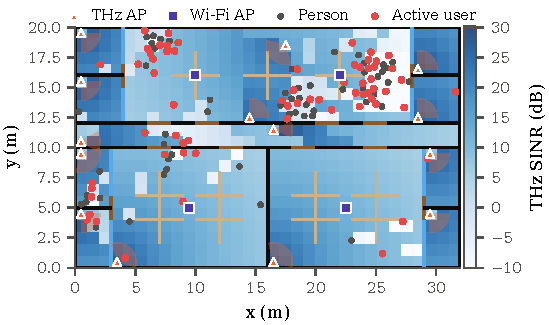
\includegraphics[width=\columnwidth]{figures/layout.pdf}
\caption{Commissioned deployment (14 THz AP sectors, 4 Wi-Fi APs) and one crowd realization (seed 0).
The background is the THz SINR of a virtual device at each 1\,m cell with this crowd present; \LayoutSeedCov\% of cells reach 5\,dB.}
\label{fig:layout}
\end{figure}

\subsection{Differences from the earlier model}
We re-implemented the model of~\cite{anon2026milp,anon2026teramove} from scratch, which revealed several defects in the original simulator; Table~\ref{tab:fixes} lists them.
The most consequential is the azimuth convention.
The MILP reports azimuths as compass bearings, but the simulator read them as mathematical angles, so APs listed at 135$^\circ$ pointed out of the building.
With the original simulator, the empty-floor coverage of the MILP layout is \LegacyCovMath\% under the mathematical reading and \LegacyCovCompass\% under the correct compass reading.
The results reported in~\cite{anon2026teramove} therefore start from a mis-oriented deployment.

\begin{table}[t]
\centering
\caption{Earlier simulator versus this work}\label{tab:fixes}
\footnotesize
\begin{tabular}{@{}p{0.43\columnwidth}p{0.49\columnwidth}@{}}
\toprule
Earlier simulator & This work\\
\midrule
Azimuth read as math angle & Compass bearing, as in~\cite{anon2026milp}\\
30\,dBi at every beamwidth & Energy-conserving gain~\eqref{eq:gain}\\
Absorption 0.05\,m$^{-1}$ (217\,dB/km) & ITU-R P.676: \AbsDbKm\,dB/km\\
Noise $-94$\,dBm in text, $-64$ in code & $N_0=\NoiseThz$\,dBm from $B$ and NF\\
Users at grid corners (on walls) & Users are people; grid at cell centres\\
Fractional density$\times$20\,dB, unbounded & Discrete bodies, exact test, capped\\
APs may cross walls & Per-room rails, Hungarian per room\\
\bottomrule
\end{tabular}
\end{table}

\subsection{Main comparison}
Table~\ref{tab:main} and Fig.~\ref{fig:main} summarize the results.
Here \MainUsers{} users are active on average.
Without adaptation, the static network satisfies \StaticS\% of users.
TeraMove reaches only \TmS\%.
Its fitness rewards grid coverage rather than served users, and it cannot use Wi-Fi.
TeraMove-H reaches \PropS$\pm$\PropSCI\%.
Re-association alone (T0) gives \PropTzero\%, and the beam stage without movement gives \NomoveS\%; the remaining gain requires moving APs.

The THz-only cascade reaches \ThzS\%, so the Wi-Fi layer adds \GainVsThz{} percentage points (pp).
At 1\,Gb/s, Wi-Fi serves about \PropWifi{} users per snapshot, because one Wi-Fi AP sustains at most \WifiMaxRate\,Gb/s.
Threshold offload reaches \NaiveS\% ($p=\NaivePS$ versus TeraMove-H); the association rule matters most at lower demand (Sec.~\ref{sec:regime}).
With the greedy instead of PACE, TeraMove-H also reaches \GreedyS\% ($p=\GreedyPS$).
At 1\,Gb/s the greedy is already optimal on every test instance (Table~\ref{tab:assoc}), so the two coincide here.

Power control switches off \PropSleep{} of the 14 APs on average and lowers total THz power from 1.40\,W to \PropPw\,W (\PowerSaving\% less).
Because all methods share random numbers, the variant without power control follows the same search and ends with the same satisfaction and displacement (\NopcS\%, \NopcDisp\,m).
Power control changes only the transmit power, as Proposition~\ref{prop:yates} guarantees.

The flat GA satisfies \GapToGa\,pp more users than TeraMove-H (\GaS\%, $p=\GaPS$).
It also moves APs \GaDisp\,m in total against \PropDisp\,m ($p=\GaPD$), so TeraMove-H moves \DispReductionVsGa\% less.
Under the same worst-case budget, neither method dominates the other: they are two points on a Pareto front (Fig.~\ref{fig:pareto}).
With PSO stages instead of GA stages, TeraMove-H reaches \HpsoS\%, and flat PSO reaches \FpsoS\%.
The GA explores the discrete beam, height and rail space better.
At equal budgets it reaches higher fitness than PSO throughout the search (Fig.~\ref{fig:conv}), so the GA is the search engine of TeraMove-H.

\begin{table}[t]
\centering
\caption{Main comparison ($\Rmin=1$\,Gb/s, 120 people, \MainSeeds{} seeds; mean, 95\% CI on $S$; Off = APs switched off)}\label{tab:main}
\footnotesize
\setlength{\tabcolsep}{3pt}
\begin{tabular}{@{}lrrrrr@{}}
\toprule
Method & $S$ (\%) & Displ. (m) & $\sum p$ (W) & Off & Evals \\
\midrule
Static & 44.8$\pm$3.1 & 0.0 & 1.40 & 0.0 & 0 \\
Wi-Fi only & 6.8$\pm$0.2 & 0.0 & 0.00 & 14.0 & 0 \\
TeraMove & 50.9$\pm$2.5 & 11.8 & 1.40 & 0.0 & 4800 \\
THz-only cascade & 77.2$\pm$2.5 & 25.8 & 0.55 & 4.2 & 6400 \\
Threshold offload & 83.0$\pm$2.8 & 23.3 & 0.51 & 4.3 & 6400 \\
Flat PSO & 78.3$\pm$2.5 & 22.4 & 0.45 & 4.4 & 6400 \\
Flat GA & 87.3$\pm$2.7 & 30.4 & 0.61 & 3.9 & 6400 \\
\midrule
w/ HPSO tiers & 75.0$\pm$2.5 & 13.5 & 0.43 & 4.5 & 6400 \\
w/ greedy assoc. & 84.4$\pm$2.6 & 24.6 & 0.53 & 4.1 & 6400 \\
w/o power ctrl & 84.4$\pm$2.6 & 24.7 & 1.40 & 0.0 & 6400 \\
w/o movement & 58.9$\pm$2.6 & 0.0 & 0.36 & 4.9 & 1600 \\
\textbf{TeraMove-H} & 84.4$\pm$2.6 & 24.7 & 0.53 & 4.0 & 6400 \\
\bottomrule
\end{tabular}

\end{table}

\begin{figure*}[t]
\centering
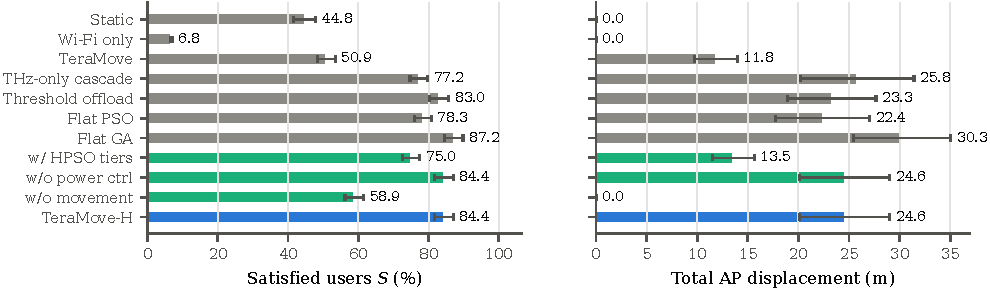
\includegraphics[width=\textwidth]{figures/main_bars.pdf}
\caption{Satisfied users and total AP displacement per method (mean and 95\% CI over \MainSeeds{} seeds).}
\label{fig:main}
\end{figure*}

\begin{figure}[t]
\centering
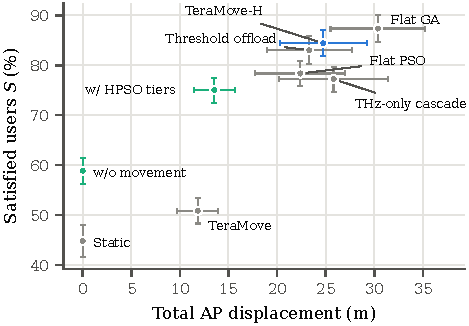
\includegraphics[width=\columnwidth]{figures/pareto.pdf}
\caption{Satisfaction versus displacement (mean, 95\% CI). The variant without power control coincides with TeraMove-H and is not shown.}
\label{fig:pareto}
\end{figure}

\begin{figure}[t]
\centering
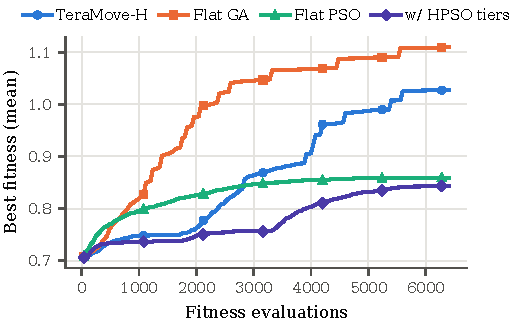
\includegraphics[width=\columnwidth]{figures/convergence.pdf}
\caption{Best fitness~\eqref{eq:fit} versus evaluations, averaged over seeds that reach the search stages.}
\label{fig:conv}
\end{figure}

\subsection{When must APs move? Demand--crowd regime}\label{sec:regime}
Fig.~\ref{fig:regime} sweeps $\Rmin\in\{0.1,0.25,0.5,1,2\}$\,Gb/s and 60--240 people.
At 0.1\,Gb/s, Wi-Fi absorbs the users whose THz links are blocked: re-association alone serves \RegimeTzeroLow\% on average, and \RegimeElecLowDemand\% of the snapshots reach $\eta$ without moving any AP.
At 2\,Gb/s, re-association serves \RegimeTzeroHigh\%, no snapshot is resolved electronically (\RegimeElecHighDemand\%), and APs must move.
Table~\ref{tab:regime} compares the association rules.
TeraMove-H with PACE beats threshold offload by \GapVsNaiveA, \GapVsNaiveB, \GapVsNaiveC{} and \GapVsNaiveD\,pp at 0.1, 0.25, 0.5 and 1\,Gb/s (all $p<10^{-3}$, Wilcoxon over seeds and crowd sizes).
At 2\,Gb/s the difference is \GapVsNaiveE\,pp and not significant ($p=\GapVsNaivePE$).
The airtime-aware association pays off when Wi-Fi capacity is a scarce resource worth allocating; at 2\,Gb/s, Wi-Fi can hardly serve anyone.

\textbf{PACE versus greedy in the full system.}
Table~\ref{tab:pace} runs the same cascade with both association algorithms on the same seeds and crowds.
T0 uses the starting geometry for both, so its difference isolates the association algorithm.
At 0.1\,Gb/s, PACE raises T0 satisfaction by \PaceTzeroGainA\,pp.
More snapshots are then resolved without any movement (\PaceElecA\% versus \GreedyElecA\%), and the mean displacement falls from \GreedyDispA\,m to \PaceDispA\,m.
The final satisfaction rises by \PaceSGainA\,pp ($p=\PaceSPA$).
The search compensates for most association errors by moving APs, so the final gains are small, and at 0.25--2\,Gb/s they are not significant ($p\ge\PaceSPMinRest$).
At 1 and 2\,Gb/s, T0 is identical, because the greedy is already optimal there.
The price is run time: a snapshot at 0.1\,Gb/s takes about \PaceRtRatioA{} times longer, because PACE runs inside every fitness evaluation.

\textbf{Certified escalation.}
In \EscN{} regime snapshots, T0 fell short of $\eta$ and TeraMove-H escalated.
In \EscCertPct\% of them, the dual bound of PACE proves that no association at the starting geometry and $\Pmax$ reaches $\eta$, so leaving T0 was necessary and not an artifact of the association heuristic.

Without Wi-Fi, satisfaction does not change with demand up to 1\,Gb/s, because a THz AP has far more capacity than its users need and only coverage limits service.
Over the whole grid, TeraMove-H moves APs \RegimeDispRatio\% less than the flat GA.

\begin{figure*}[t]
\centering
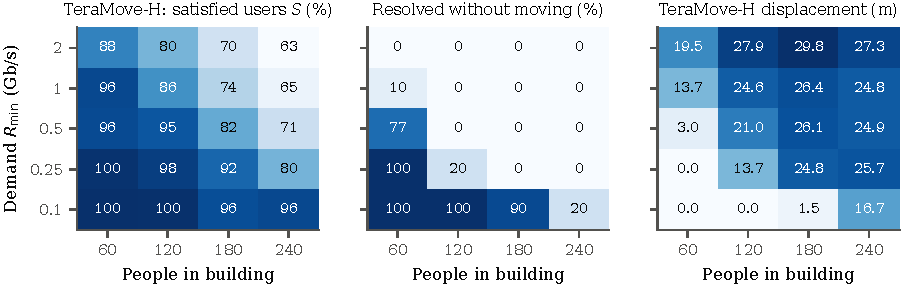
\includegraphics[width=\textwidth]{figures/regime.pdf}
\caption{Regime map (mean over \MainSeeds{} seeds per cell): satisfaction of TeraMove-H, share of snapshots resolved without any movement, and TeraMove-H displacement.}
\label{fig:regime}
\end{figure*}

\begin{table}[t]
\centering
\caption{Satisfaction and displacement versus demand (mean over crowd sizes and seeds)}\label{tab:regime}
\footnotesize
\setlength{\tabcolsep}{3pt}
\begin{tabular}{@{}lrrrrr@{}}
\toprule
$R_{\min}$ (Gb/s) & 0.1 & 0.25 & 0.5 & 1 & 2 \\
\midrule
THz-only cascade $S$ (\%) & 75.6 & 75.6 & 75.6 & 75.6 & 75.6 \\
Threshold offload $S$ (\%) & 96.5 & 90.5 & 84.6 & 79.5 & 75.2 \\
TeraMove-H $S$ (\%) & 98.3 & 92.5 & 86.1 & 80.4 & 75.1 \\
Flat GA $S$ (\%) & 98.9 & 94.3 & 88.4 & 83.4 & 78.0 \\
TeraMove-H displ. (m) & 3.8 & 15.5 & 19.1 & 22.3 & 25.8 \\
Flat GA displ. (m) & 5.3 & 19.8 & 25.3 & 29.8 & 33.0 \\
\bottomrule
\end{tabular}

\end{table}

\subsection{Temporal operation}
In each seed, the crowd evolves over \TEpochs{} epochs: clusters drift 1.5\,m per epoch and people keep their identity.
Each method starts every epoch from its previous configuration (Fig.~\ref{fig:temporal}).
Over all epochs, TeraMove-H satisfies \TPropS\% of users with \TPropCum\,m of cumulative movement.
The flat GA satisfies \TGaS\% with \TGaCum\,m, TeraMove \TTmS\%, and the static network \TStaticS\%.
Among users served in consecutive epochs, \TPropHo\% change their serving AP under TeraMove-H, and \TPropHv\% switch between THz and Wi-Fi.

\begin{figure}[t]
\centering
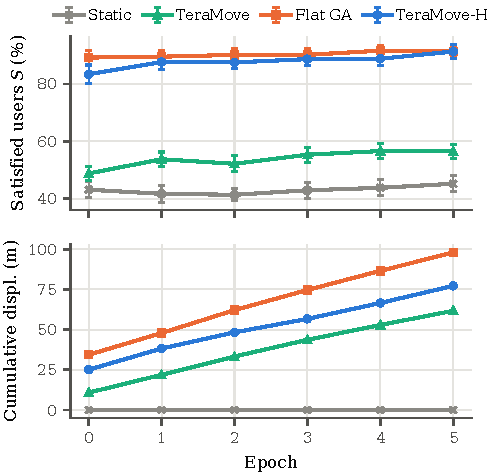
\includegraphics[width=\columnwidth]{figures/temporal.pdf}
\caption{Satisfaction per epoch (top, mean and 95\% CI) and mean cumulative displacement (bottom) under a drifting crowd.}
\label{fig:temporal}
\end{figure}

\subsection{Association optimality and sensing error}\label{sec:assoc}
We compare the greedy and PACE with the exact integer program on \AssocInstances{} instances: four crowd sizes (60--240 people), five demands, and three AP configurations per seed (commissioned and two random perturbations), over \MainSeeds{} seeds.
PACE reaches the exact optimum in \AssocPaceOptimalPct\% of instances, against \AssocOptimalPct\% for the greedy (Table~\ref{tab:assoc}).
Summed over all instances, the greedy serves \AssocShortGreedy{} users fewer than the optimum and PACE \AssocShortPace, i.e., PACE removes \AssocShortReduction\% of the shortfall.
PACE serves more users than the greedy in \AssocWins{} instances and fewer in none.
Its worst instance is \AssocPaceMaxGapText{} short (\AssocPaceWorstRatio\% of the optimum), against \AssocMaxGapText{} (\AssocWorstRatio\%) for the greedy.
PACE certifies its own optimality in \AssocCertPct\% of instances, and every certificate is correct.
The slot cuts are what make the certificate useful.
The floor of the plain linear relaxation equals the optimum in only \AssocLpTightPct\% of instances, but with slot cuts it does so in \AssocLpSlotTightPct\%, and it is never more than \AssocLpSlotMaxGap{} users above the optimum.
The greedy errs only at low demand, where an AP holds many users.
Median run times are \AssocTGreedy\,ms for the greedy, \AssocTPace\,ms for PACE and \AssocTExact\,ms for the exact solver (99th percentiles \AssocTGreedyPnn, \AssocTPacePnn{} and \AssocTExactPnn\,ms; all instances solved in parallel on 22 cores).

\begin{table}[t]
\centering
\caption{Association versus the exact optimum (\AssocPerDemand{} instances per demand)}\label{tab:assoc}
\footnotesize
\setlength{\tabcolsep}{3pt}
\begin{tabular}{@{}lrrrrr@{}}
\toprule
$R_{\min}$ (Gb/s) & 0.1 & 0.25 & 0.5 & 1 & 2 \\
\midrule
Greedy optimal (\%) & 56.7 & 74.7 & 89.2 & 100.0 & 100.0 \\
PACE optimal (\%) & 97.2 & 99.7 & 100.0 & 100.0 & 100.0 \\
PACE certified (\%) & 56.4 & 70.6 & 84.7 & 100.0 & 100.0 \\
Users short, greedy & 320 & 123 & 40 & 0 & 0 \\
Users short, PACE & 11 & 1 & 0 & 0 & 0 \\
\bottomrule
\end{tabular}

\end{table}

\begin{table}[t]
\centering
\caption{TeraMove-H with PACE / with greedy association (mean over crowd sizes and seeds)}\label{tab:pace}
\footnotesize
\setlength{\tabcolsep}{2pt}
\begin{tabular}{@{}lrrrrr@{}}
\toprule
$R_{\min}$ (Gb/s) & 0.1 & 0.25 & 0.5 & 1 & 2 \\
\midrule
T0 $S$ (\%) & 94.2/93.2 & 73.2/72.8 & 60.8/60.3 & 48.7/48.7 & 41.7/41.7 \\
Final $S$ (\%) & 98.3/98.0 & 92.5/92.4 & 86.1/85.9 & 80.4/80.3 & 75.1/75.2 \\
No movement (\%) & 80/78 & 33/30 & 20/19 & 2/2 & 0/0 \\
Displ. (m) & 3.8/4.5 & 15.5/16.1 & 19.1/18.7 & 22.3/22.4 & 25.8/26.1 \\
\bottomrule
\end{tabular}

\end{table}

TeraMove-H assumes that people's positions are sensed, for example by LiDAR~\cite{anon2026teramove}.
We perturb the optimizer's view of every position by Gaussian noise of standard deviation $\sigma$ and evaluate on the true crowd (Fig.~\ref{fig:sensing}).
Satisfaction is \SensZero, \SensQuarter, \SensHalf{} and \SensOne\% for $\sigma=0$, 0.25, 0.5 and 1\,m.
Even with 1\,m error, the search beats re-association alone (\PropTzero\%), but the sensitivity is high.
A 0.4\,m-wide body decides whether a THz link exists, so a configuration tuned to a slightly wrong crowd can place beams exactly behind people.
TeraMove-H therefore needs decimetre-level context, or a search that is robust to position error (future work).

\begin{figure}[t]
\centering
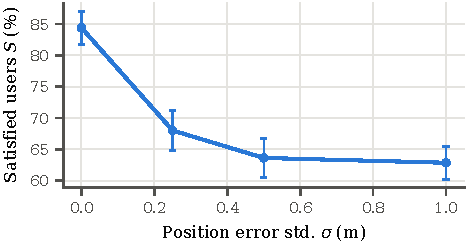
\includegraphics[width=\columnwidth]{figures/sensing.pdf}
\caption{Sensitivity of TeraMove-H to position-sensing error (mean, 95\% CI).}
\label{fig:sensing}
\end{figure}

\section{Discussion and Limitations}
\textbf{Exposure.}
The largest THz EIRP is \MaxEirp\,dBm ($\alpha=30^\circ$), which gives \ExposureHalfMeter\,W/m$^2$ at 0.5\,m.
This is below the ICNIRP 2020 general-public whole-body reference level of 10\,W/m$^2$ for 2--300\,GHz~\cite{icnirp2020}, so exposure does not constrain power here.
\textbf{Model scope.}
Links are line-of-sight only; specular reflections would add paths and raise every method's satisfaction.
Interference assumes that every AP that is switched on transmits continuously, which is pessimistic.
The Wi-Fi model uses median path loss without shadow fading.
The sensing study perturbs only positions; device orientation is assumed known.
\textbf{Mechanics.}
At an assumed rail speed of 0.2\,m/s, the largest single-AP move of TeraMove-H takes \PropLat\,s on average, so the mechanical stage suits scheduled rather than per-second adaptation.
\textbf{Search.}
Under an equal budget, the flat GA attains higher satisfaction at the cost of more movement.
An operator who values satisfaction over movement can lower $\beta$ or skip stage T2.

\section{Conclusion}
TeraMove-H extends movable THz AP reconfiguration to a hybrid THz/Wi-Fi network with airtime-aware association and minimum-power control.
Relative to the static deployment, it raises the share of satisfied users by \GainVsStatic\,pp at 1\,Gb/s, and it cuts THz transmit power by \PowerSaving\%.
Its association algorithm, PACE, reaches the exact optimum in \AssocPaceOptimalPct\% of test instances, and it can prove when re-association alone cannot reach the target, so APs move only when needed.
Wi-Fi offload makes physical movement unnecessary at low demand, while at multi-gigabit demand movement remains essential.
The re-implementation also corrected several defects of the earlier simulator, and all results here come from runs of the corrected model.

\bibliographystyle{IEEEtran}
\bibliography{refs}

\end{document}
